\documentclass[12 pt]{article}
\usepackage{amsfonts, amssymb, amsmath, graphicx}

\oddsidemargin=-0.5cm                 	
\setlength{\textwidth}{6.5in}         	
\addtolength{\voffset}{-20pt}        		
\addtolength{\headsep}{25pt}      
\setlength{\parindent}{0pt}

\pagestyle{myheadings}                           
\markright{Lixi Zhang\hfill Homework 1 \hfill Algorithm Design\hfill }

\newcommand{\eqn}[0]{\begin{array}{rcl}}
\newcommand{\eqnend}[0]{\end{array} }

\newcommand{\qed}[0]{$\square$}

\begin{document}

\section{Problem 7}

\textbf{Statement: } We are given $n$ balls and $n$ bins. Each ball is thrown into a random bin(each bin is chosen with probability $1/n$). Prove that:

$$
\lim_{n\to +\infty}\mathbb{E}\left[\frac{the\ number\ of\ empty\ bins}{n}\right] = \frac{1}{e}
$$

where $e$ is the base of the natural logarithm.

\textbf{Proof: }

By the linearity of expectation:

$$
\lim_{n\to +\infty}\mathbb{E}\left[\frac{the\ number\ of\ empty\ bins}{n}\right]
$$

equals to

$$
\lim_{n\to +\infty}\mathbb{E}\left[X\right]
$$

$X$ equals to $1$ if a bin is empty after this procession and $0$ otherwise.

This is equivalent to

$$
\lim_{n\to +\infty}(1 - \frac{1}{n})^n = \frac{1}{e}
$$

\section{Problem 8}

\textbf{Statement: } For two women $w$ and $w'$, we write $w <_m w'$ to denote that $w$ is worse than $w'$ in the preference list of man $m$. Given two stable matchings $f$ and $f'$(You can easily construct an example in with there are multiple stable matchings), define a mapping $g = f\vee f'$ as follows:

\begin{enumerate}
  \item for each man $m$, assign him more preferred partner
  $$
  g(m) = f(m)\ \text{if}\ f(m) \ge_m f'(m)
  $$
  $$
  g(m) = f'(m)\ \text{if}\ f'(m) >_m f(m)
  $$
  \item for each woman $w$, assign her less preferred partner
  $$
  g(w) = f(w)\ \text{if}\ f(w)\le_w f'(w)
  $$
  $$
  g(w) = f'(w)\ \text{if}\ f'(w)<_w f(w)
  $$
\end{enumerate}

Show that if both $f$ and $f'$ are stable matchings, so is $g$. (noto: We can similarly define $f\wedge f'$. Then all stable matchings form a distributive lattice, an abstract yet very popular object studied in combinatorics.)

\textbf{Proof: }

First, $f(m) = f'(m), f(w) = f'(w)$ is trivial. Let's skip this case.

Then we can observe that these two matchings form an undirected graph with circles(Nodes denote men and women. Each node's degree is $2$.)

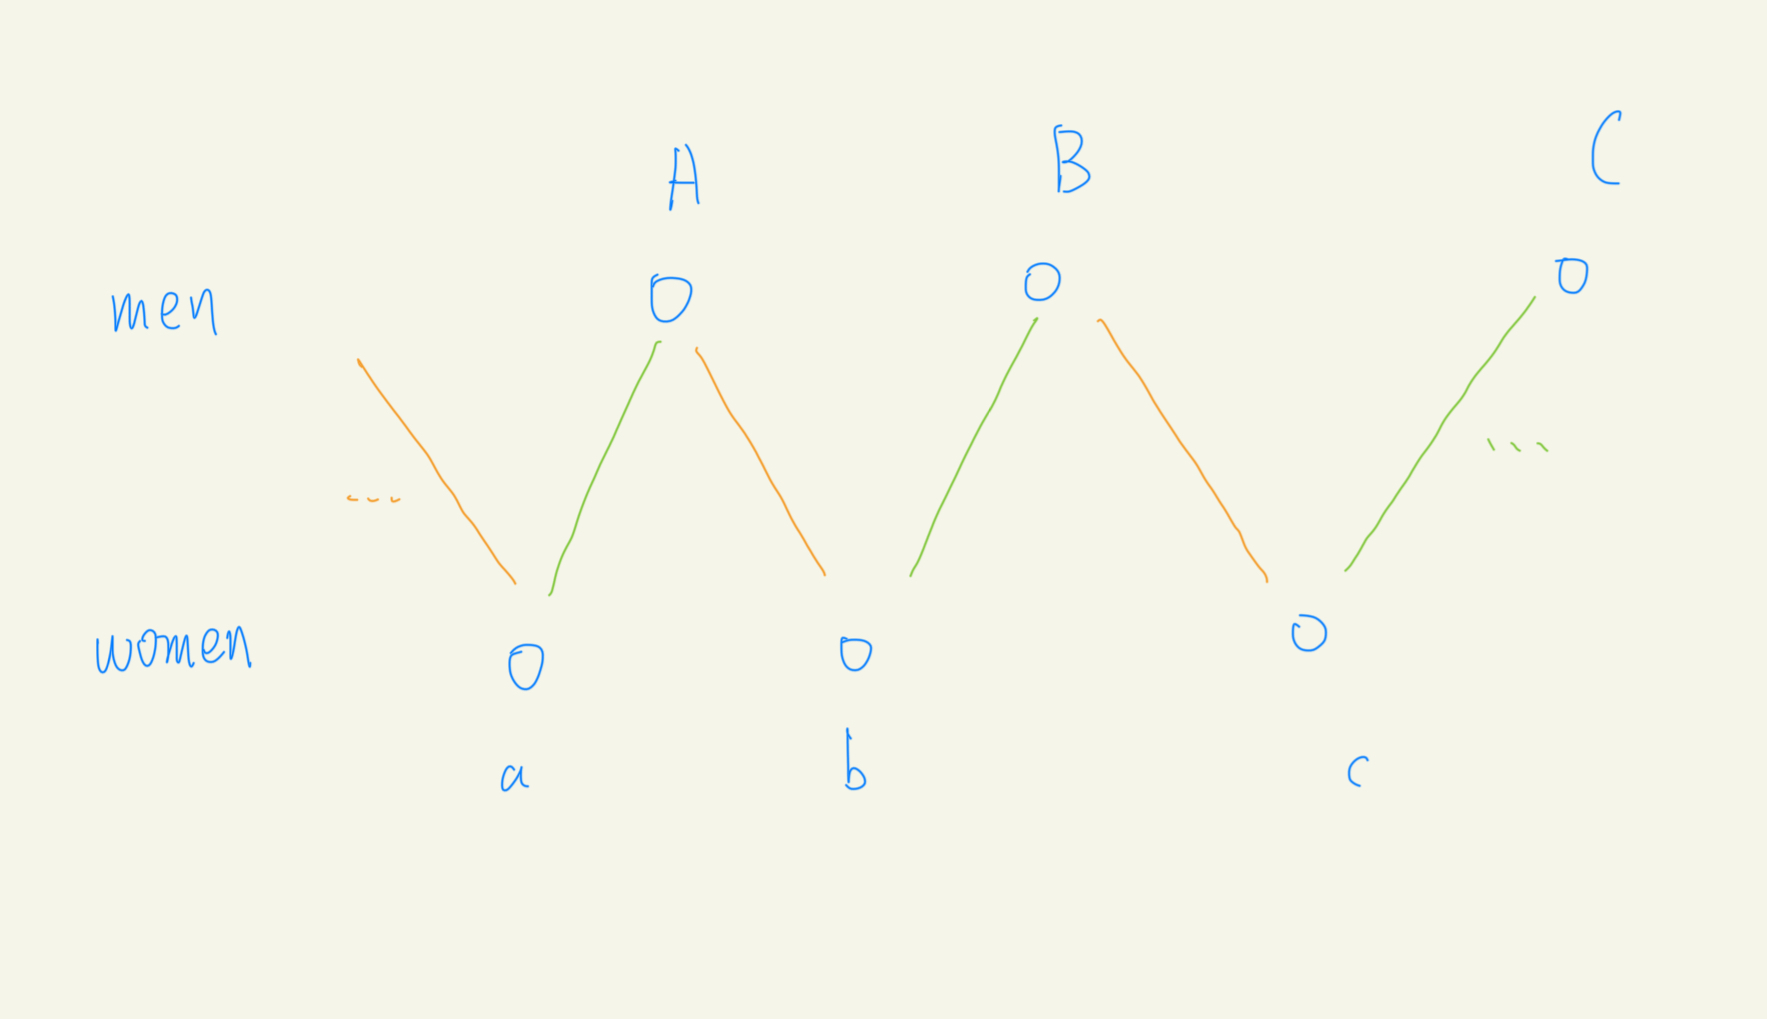
\includegraphics[width=\linewidth]{P8_1.jpeg}

Assume that $A$ prefers $b$ than $a$.

$b$ must prefer $B$ to $A$, otherwise $(A, a), (B, b)$ are not stable matchings because of $(A, b)$.

Also, $B$ must prefer $c$ to $b$, otherwise $(A, b), (B, c)$ are not stable matchings because of $(B, b)$.

Thus, according to the statement, $g$ is a stable matching which equals to the orange one.

This is because we have assumed that $A$ prefers $b$ than $a$. Likewise, if we consider $A$ prefers $a$ than $b$, we can get silimar conclusion. This shows that an undirected circle infers two directions(ways) of matchings.

\section{Problem 9}

\textbf{Statement: } As we mentioned, there could be multiple stable matchings. The Gale-Shapley algorithm only finds one such stable matching. For any man $m$, let $best(m)$ be the best woman matched to $m$ in all possible stable matchings. Show that Gale-Shapley algorithm is man-optimal, in the sense that it returns a stable matching where for any $m$, $m$ is matched to $best(m)$.(If we let women propose, the resulting matching is women-optimal)

\textbf{Proof: } 

Consider a man $m$ matches $w$ by Gale-Shapley algorithm, and $m$ matches $w'$ in some stable matching $S$.($w' >_m w$)

According to the process of GS, when $w'$ refuses $m$, she has already matches $m'$ and $m' >_w m$.

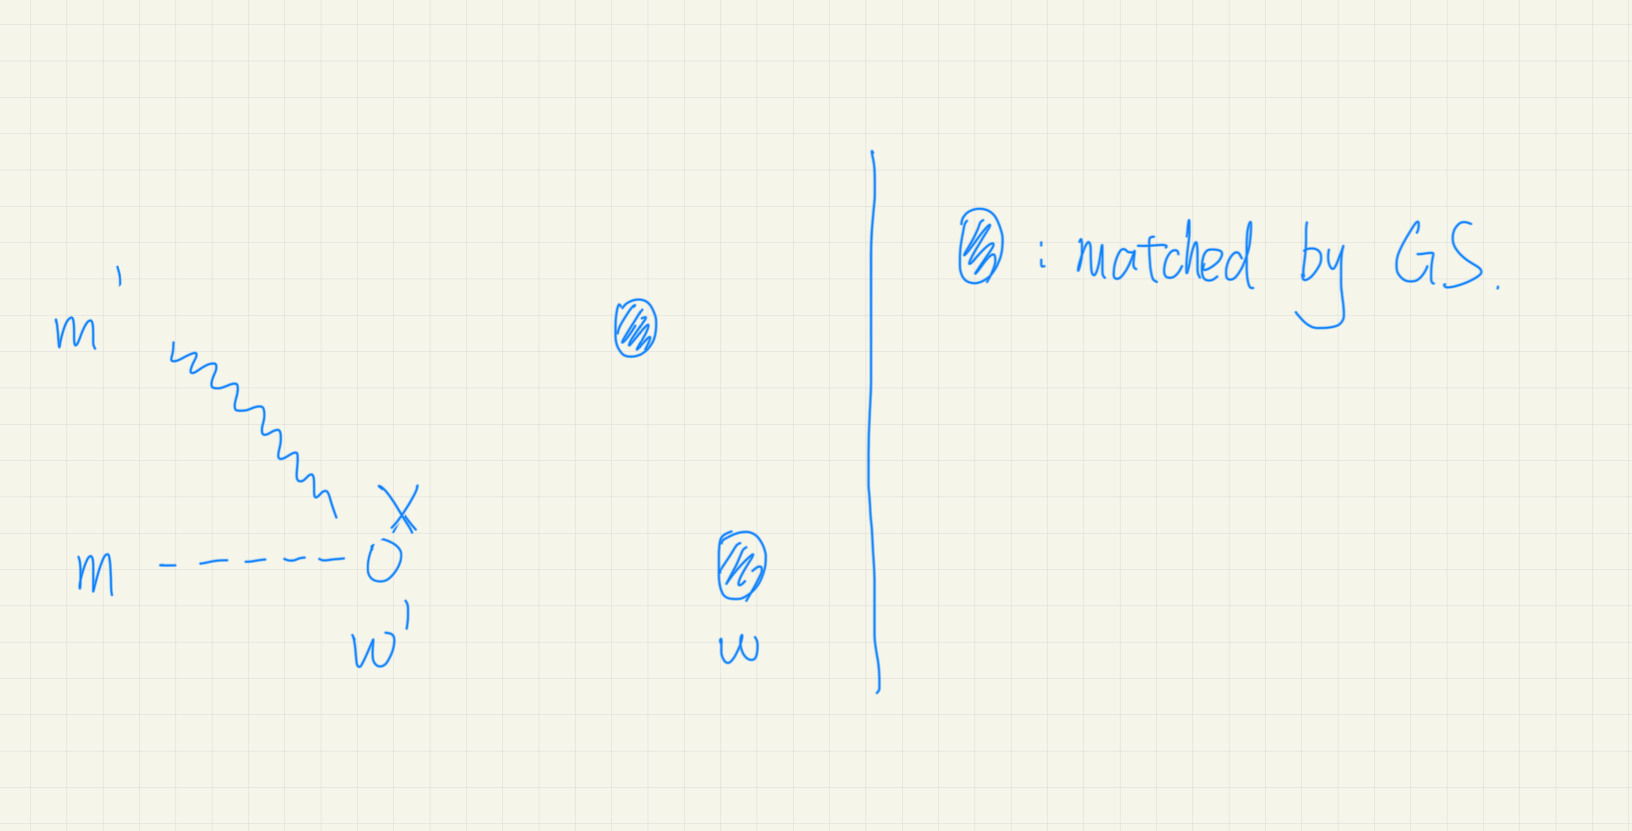
\includegraphics[width=\linewidth]{P9_1.jpeg}

No matter who $m'$ matches at last, we can infer that $(m', w')$ may cause unstable matching if $m'$ matches a woman worse than $w'$ in $S$.

Also, we have $w' \ge_{m'} f(m')$(let $f(m)$ denote the woman matched by GS).

So we can simply mark $w'$ visited and recursively consider the same problem for $m'$(That we means $w'$ can't be matched to others because we need $(m, w')$). But we can't recur forever. So it contradicts.

\end{document}